\documentclass{beamer}\usepackage[]{graphicx}\usepackage[]{xcolor}
% maxwidth is the original width if it is less than linewidth
% otherwise use linewidth (to make sure the graphics do not exceed the margin)
\makeatletter
\def\maxwidth{ %
  \ifdim\Gin@nat@width>\linewidth
    \linewidth
  \else
    \Gin@nat@width
  \fi
}
\makeatother

\definecolor{fgcolor}{rgb}{0.345, 0.345, 0.345}
\newcommand{\hlnum}[1]{\textcolor[rgb]{0.686,0.059,0.569}{#1}}%
\newcommand{\hlstr}[1]{\textcolor[rgb]{0.192,0.494,0.8}{#1}}%
\newcommand{\hlcom}[1]{\textcolor[rgb]{0.678,0.584,0.686}{\textit{#1}}}%
\newcommand{\hlopt}[1]{\textcolor[rgb]{0,0,0}{#1}}%
\newcommand{\hlstd}[1]{\textcolor[rgb]{0.345,0.345,0.345}{#1}}%
\newcommand{\hlkwa}[1]{\textcolor[rgb]{0.161,0.373,0.58}{\textbf{#1}}}%
\newcommand{\hlkwb}[1]{\textcolor[rgb]{0.69,0.353,0.396}{#1}}%
\newcommand{\hlkwc}[1]{\textcolor[rgb]{0.333,0.667,0.333}{#1}}%
\newcommand{\hlkwd}[1]{\textcolor[rgb]{0.737,0.353,0.396}{\textbf{#1}}}%
\let\hlipl\hlkwb

\usepackage{framed}
\makeatletter
\newenvironment{kframe}{%
 \def\at@end@of@kframe{}%
 \ifinner\ifhmode%
  \def\at@end@of@kframe{\end{minipage}}%
  \begin{minipage}{\columnwidth}%
 \fi\fi%
 \def\FrameCommand##1{\hskip\@totalleftmargin \hskip-\fboxsep
 \colorbox{shadecolor}{##1}\hskip-\fboxsep
     % There is no \\@totalrightmargin, so:
     \hskip-\linewidth \hskip-\@totalleftmargin \hskip\columnwidth}%
 \MakeFramed {\advance\hsize-\width
   \@totalleftmargin\z@ \linewidth\hsize
   \@setminipage}}%
 {\par\unskip\endMakeFramed%
 \at@end@of@kframe}
\makeatother

\definecolor{shadecolor}{rgb}{.97, .97, .97}
\definecolor{messagecolor}{rgb}{0, 0, 0}
\definecolor{warningcolor}{rgb}{1, 0, 1}
\definecolor{errorcolor}{rgb}{1, 0, 0}
\newenvironment{knitrout}{}{} % an empty environment to be redefined in TeX

\usepackage{alltt}
%% Possible paper sizes: a0, a0b, a1, a2, a3, a4.
%% Possible orientations: portrait, landscape
%% Font sizes can be changed using the scale option.
\usepackage[size = a0,orientation=portrait,scale=1.5]{beamerposter}

% Theme
\usetheme{LLT-poster}
% \usecolortheme{ComingClean}
\usecolortheme{Entrepreneur}
% \usecolortheme{ConspiciousCreep}  %% VERY garish.

% Packages
\usepackage[utf8]{inputenc}
\usepackage[T1]{fontenc}
\usepackage{libertine}
\usepackage[scaled=0.92]{inconsolata}
\usepackage[libertine]{newtxmath}
\usepackage{booktabs} % for styling kable-Latex tables
\usepackage[most]{tcolorbox} % for blocks of same height w/ tcolorbox

% Margins
% \setbeamersize{text margin left=30mm,text margin right=50mm}

% Research Info
\author[e.costantini@tilburguniversity.edu]{Edoardo Costantini}
\title{Solving the `many variables' problem in MICE with supervised principal component regression}
\institute{Tilburg University, Netherlands}
% Optional foot image
% \footimage{
\includegraphics[width=4cm]{images/qrcode.png}}
\IfFileExists{upquote.sty}{\usepackage{upquote}}{}
\begin{document}

% Read R material


% What begins here?
\begin{frame}[fragile]\centering

% Intro statement --------------------------------------------------------------

\begin{columns}[c]
  \begin{column}{.46\textwidth}

    \begin{block}{In one sentence}
      \vspace{2.05cm}
      \Large Using \textbf{supervised principal component regression} as a univariate \textbf{imputation} model in \textbf{MICE} is a great way to solve the \textbf{many-variables} imputation problem.
      \vspace{2.05cm}
      \end{block}
    
  \end{column}  

  \begin{column}{.46\textwidth}

  % Block 1
  \begin{block}{Large data with missing values (-)}
\begin{knitrout}
\definecolor{shadecolor}{rgb}{0.969, 0.969, 0.969}\color{fgcolor}\begin{table}
\centering
\begin{tabular}[t]{lrccccccccccccc}
\toprule
  & $x_1$ & $x_2$ & $x_3$ & $x_4$ & ... & $w_{141}$ & $w_{142}$ & $w_{143}$ & $w_{144}$ & ... & $z_{(p-3)}$ & $z_{(p-2)}$ & $z_{(p-1)}$ & $z_p$\\
\midrule
Esther & 3 & - & 4 & 6 &  & 7 & 6 & 2 & 2 &  & 5 & 4 & 9 & 8\\
Anton & - & - & 3 & 1 &  & 8 & 3 & 7 & 10 &  & 8 & 10 & 3 & 7\\
Leonie & - & 7 & - & 4 &  & 5 & 9 & 3 & 6 &  & 9 & 10 & 9 & 2\\
Joran & 1 & 4 & 4 & - &  & 9 & 1 & 5 & 5 &  & 3 & 1 & 9 & 8\\
... &  &  &  &  &  &  &  &  &  &  &  &  &  & \\
\addlinespace
Mihai & - & 8 & - & 4 &  & 10 & 6 & 2 & 9 &  & 2 & 5 & 2 & 10\\
\bottomrule
\end{tabular}
\end{table}

\end{knitrout}
  \end{block}

  \end{column}

  \end{columns}

  \bigskip
  \bigskip

% Section 2: Approaches --------------------------------------------------------

\begin{columns}[T]
\begin{column}{.42\textwidth}

% Block 2
\begin{block}{Expert imputation model specification}

  \begin{itemize}
      \item Remove constants and collinear variables.
      \item Evaluate connection between variables in the data.
      \item Apply a correlation-threshold selection.
      \item Extra: use total scores for item scales.
      \item Extra: use single measurement in longitudinal data.
  \end{itemize}

\end{block}

\end{column}

\begin{column}{.06\textwidth}
  \vspace{5cm}
  \begin{center}
    \huge \textbf{VS}
    \end{center}

  \end{column}

\begin{column}{.42\textwidth}

% Block 3
\begin{block}{Automatic imputation model specification}

  \begin{itemize}
    \item MICE with Principal component regression (MI-PCR)
    \item MICE with Association-threshold supervised principal component regression (MI-SPCR)
    \item MICE with Principal covariates regression (MI-PCovR)
    \item MICE with Partial least square (MI-PLSR)
  \end{itemize}

\end{block}

\end{column}

\end{columns}

\bigskip
{\usebeamercolor[bg]{headline}\hrulefill}
\bigskip

% Section 3: Plots -------------------------------------------------------------

\begin{columns}

  % First column

  \begin{column}{.46\textwidth}
    \begin{block}{Percent relative bias}

      \begin{figure}
        \centering
\begin{knitrout}
\definecolor{shadecolor}{rgb}{0.969, 0.969, 0.969}\color{fgcolor}

{\centering 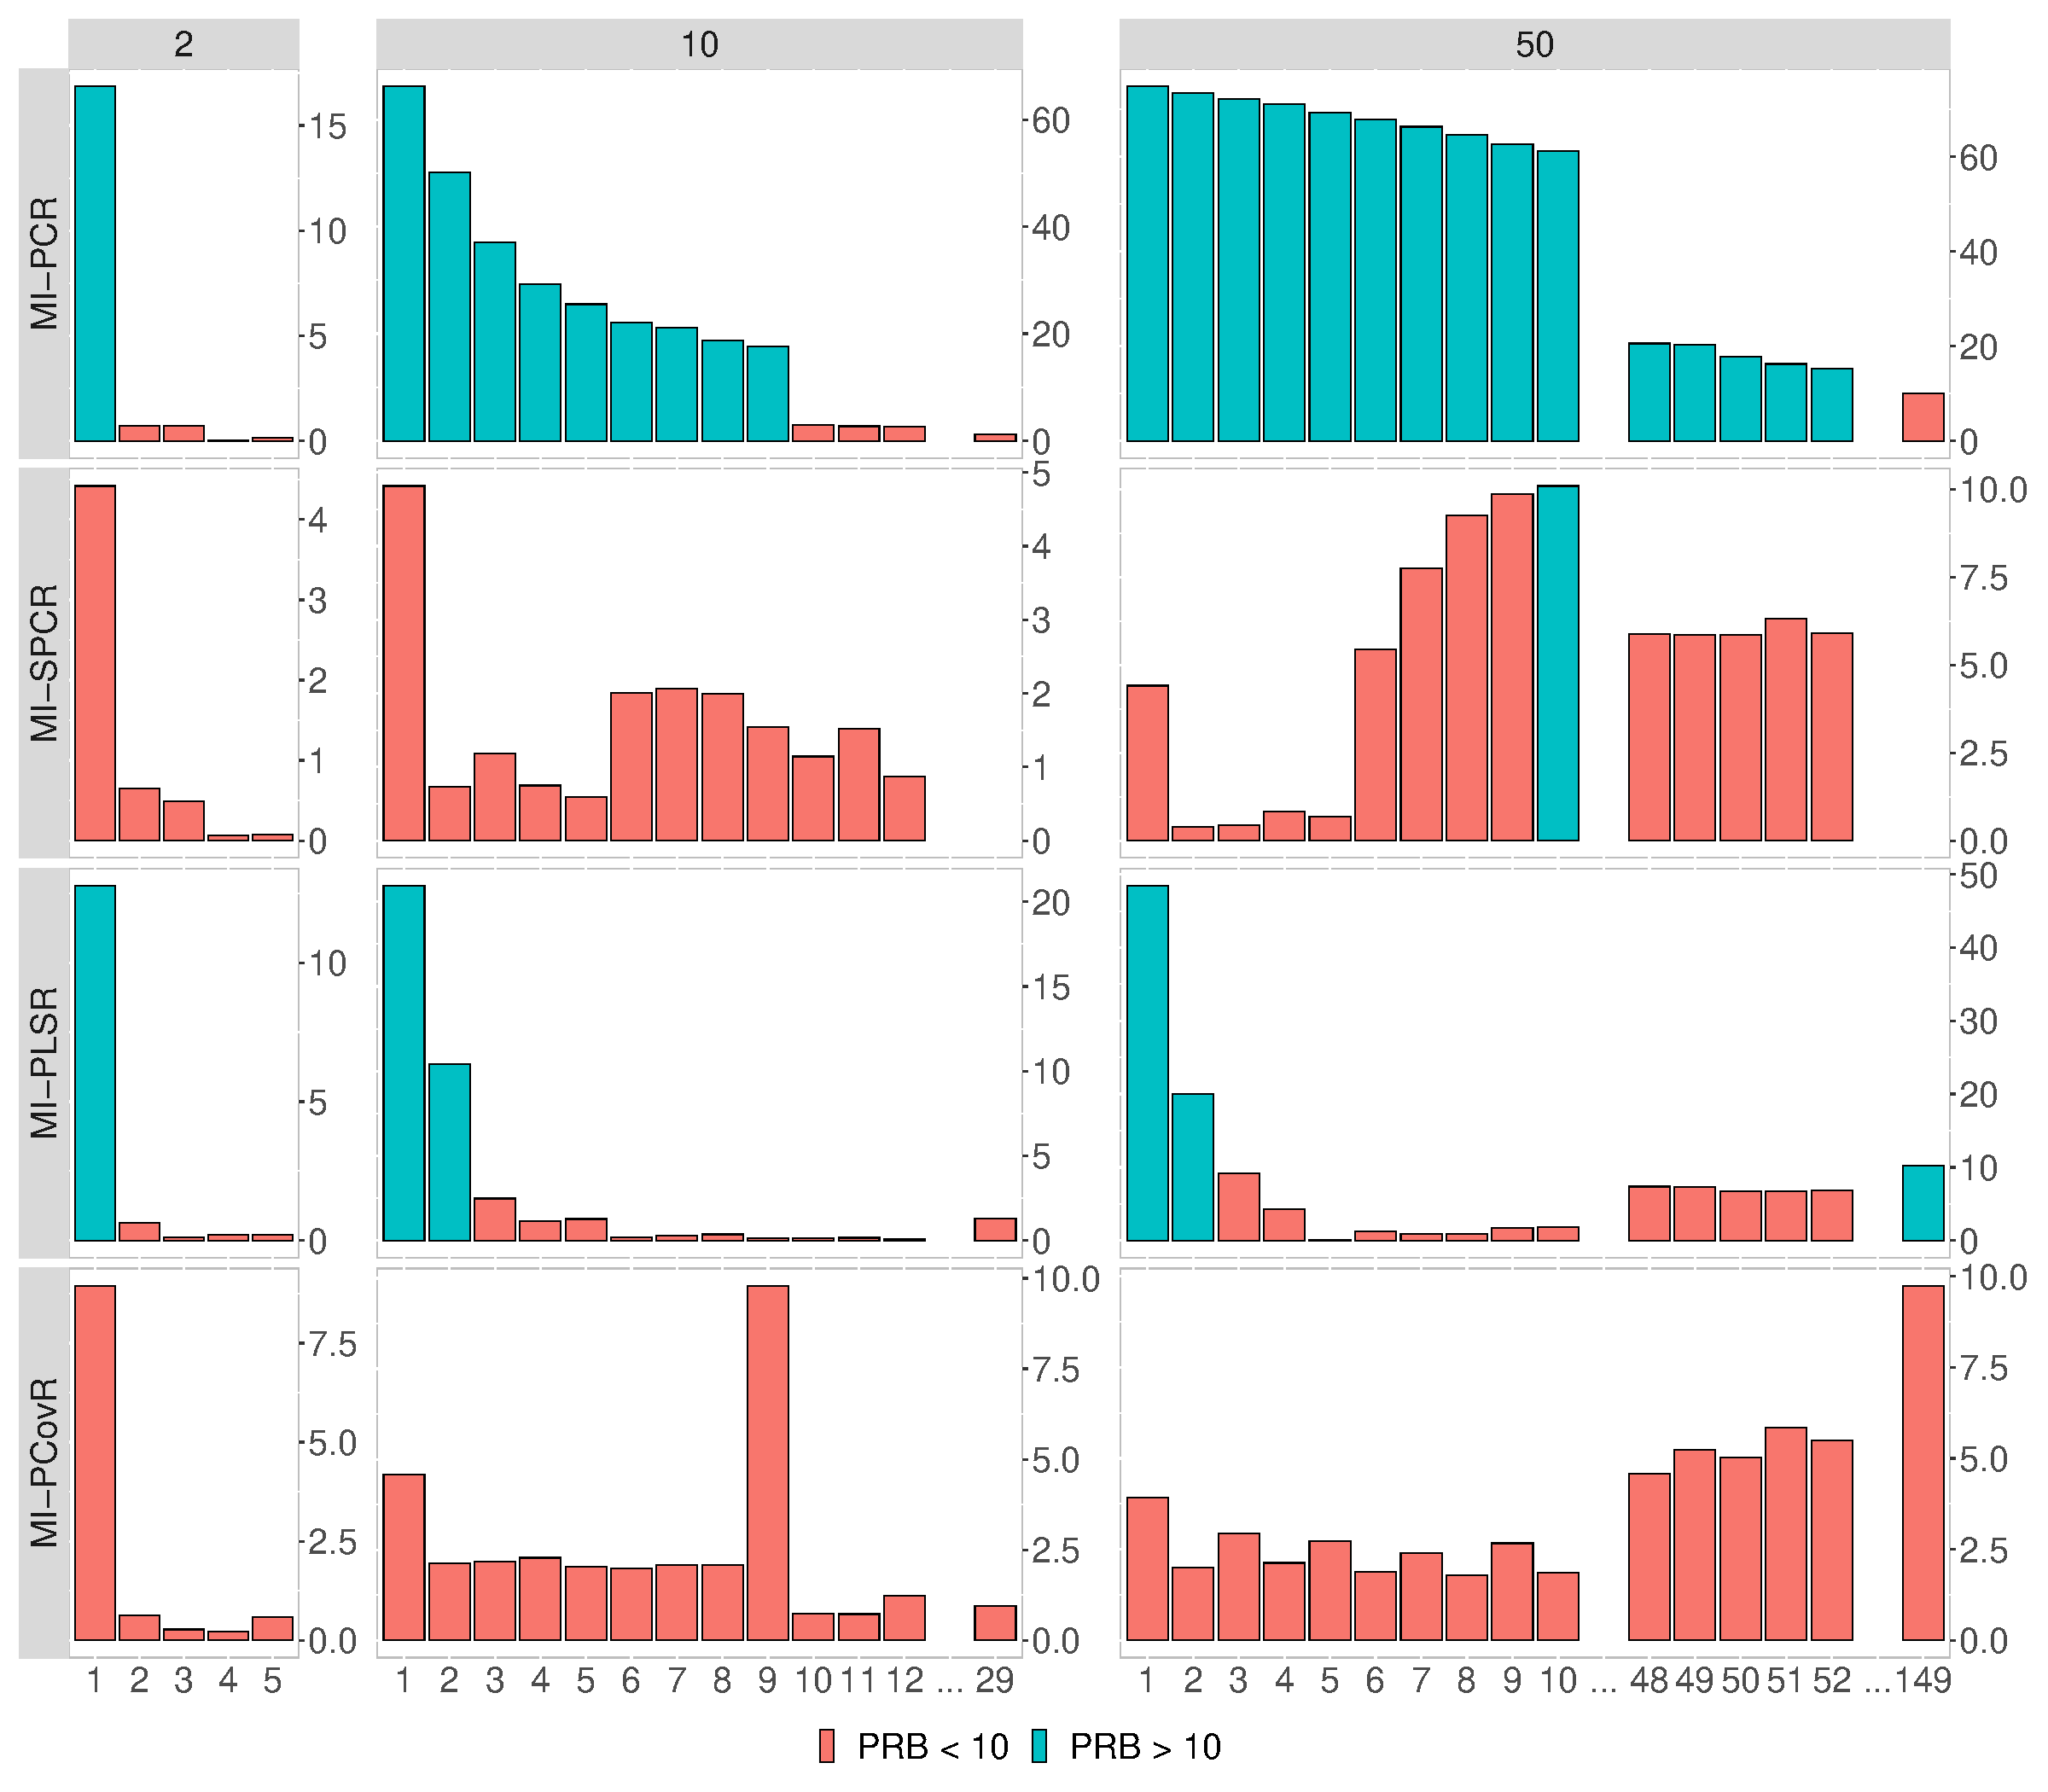
\includegraphics[width=\maxwidth]{figure/plot-prb-1} 

}


\end{knitrout}
          \caption{
            \label{fig:prb-text} 
            The percent relative bias (Y-axis) for the correlation coefficient between $x_1$ and $x_2$, obtained after imputing the missing values with the four PCR-based imputation methods (grid rows), is reported as a function of the number of components used (X-axis).
            }
        \end{figure}
        
    \end{block}
    
  \end{column}  

  % Second column

  \begin{column}{.46\textwidth}

    \begin{block}{Confidence interval coverage}
      
      \begin{figure}
        \centering
\begin{knitrout}
\definecolor{shadecolor}{rgb}{0.969, 0.969, 0.969}\color{fgcolor}

{\centering 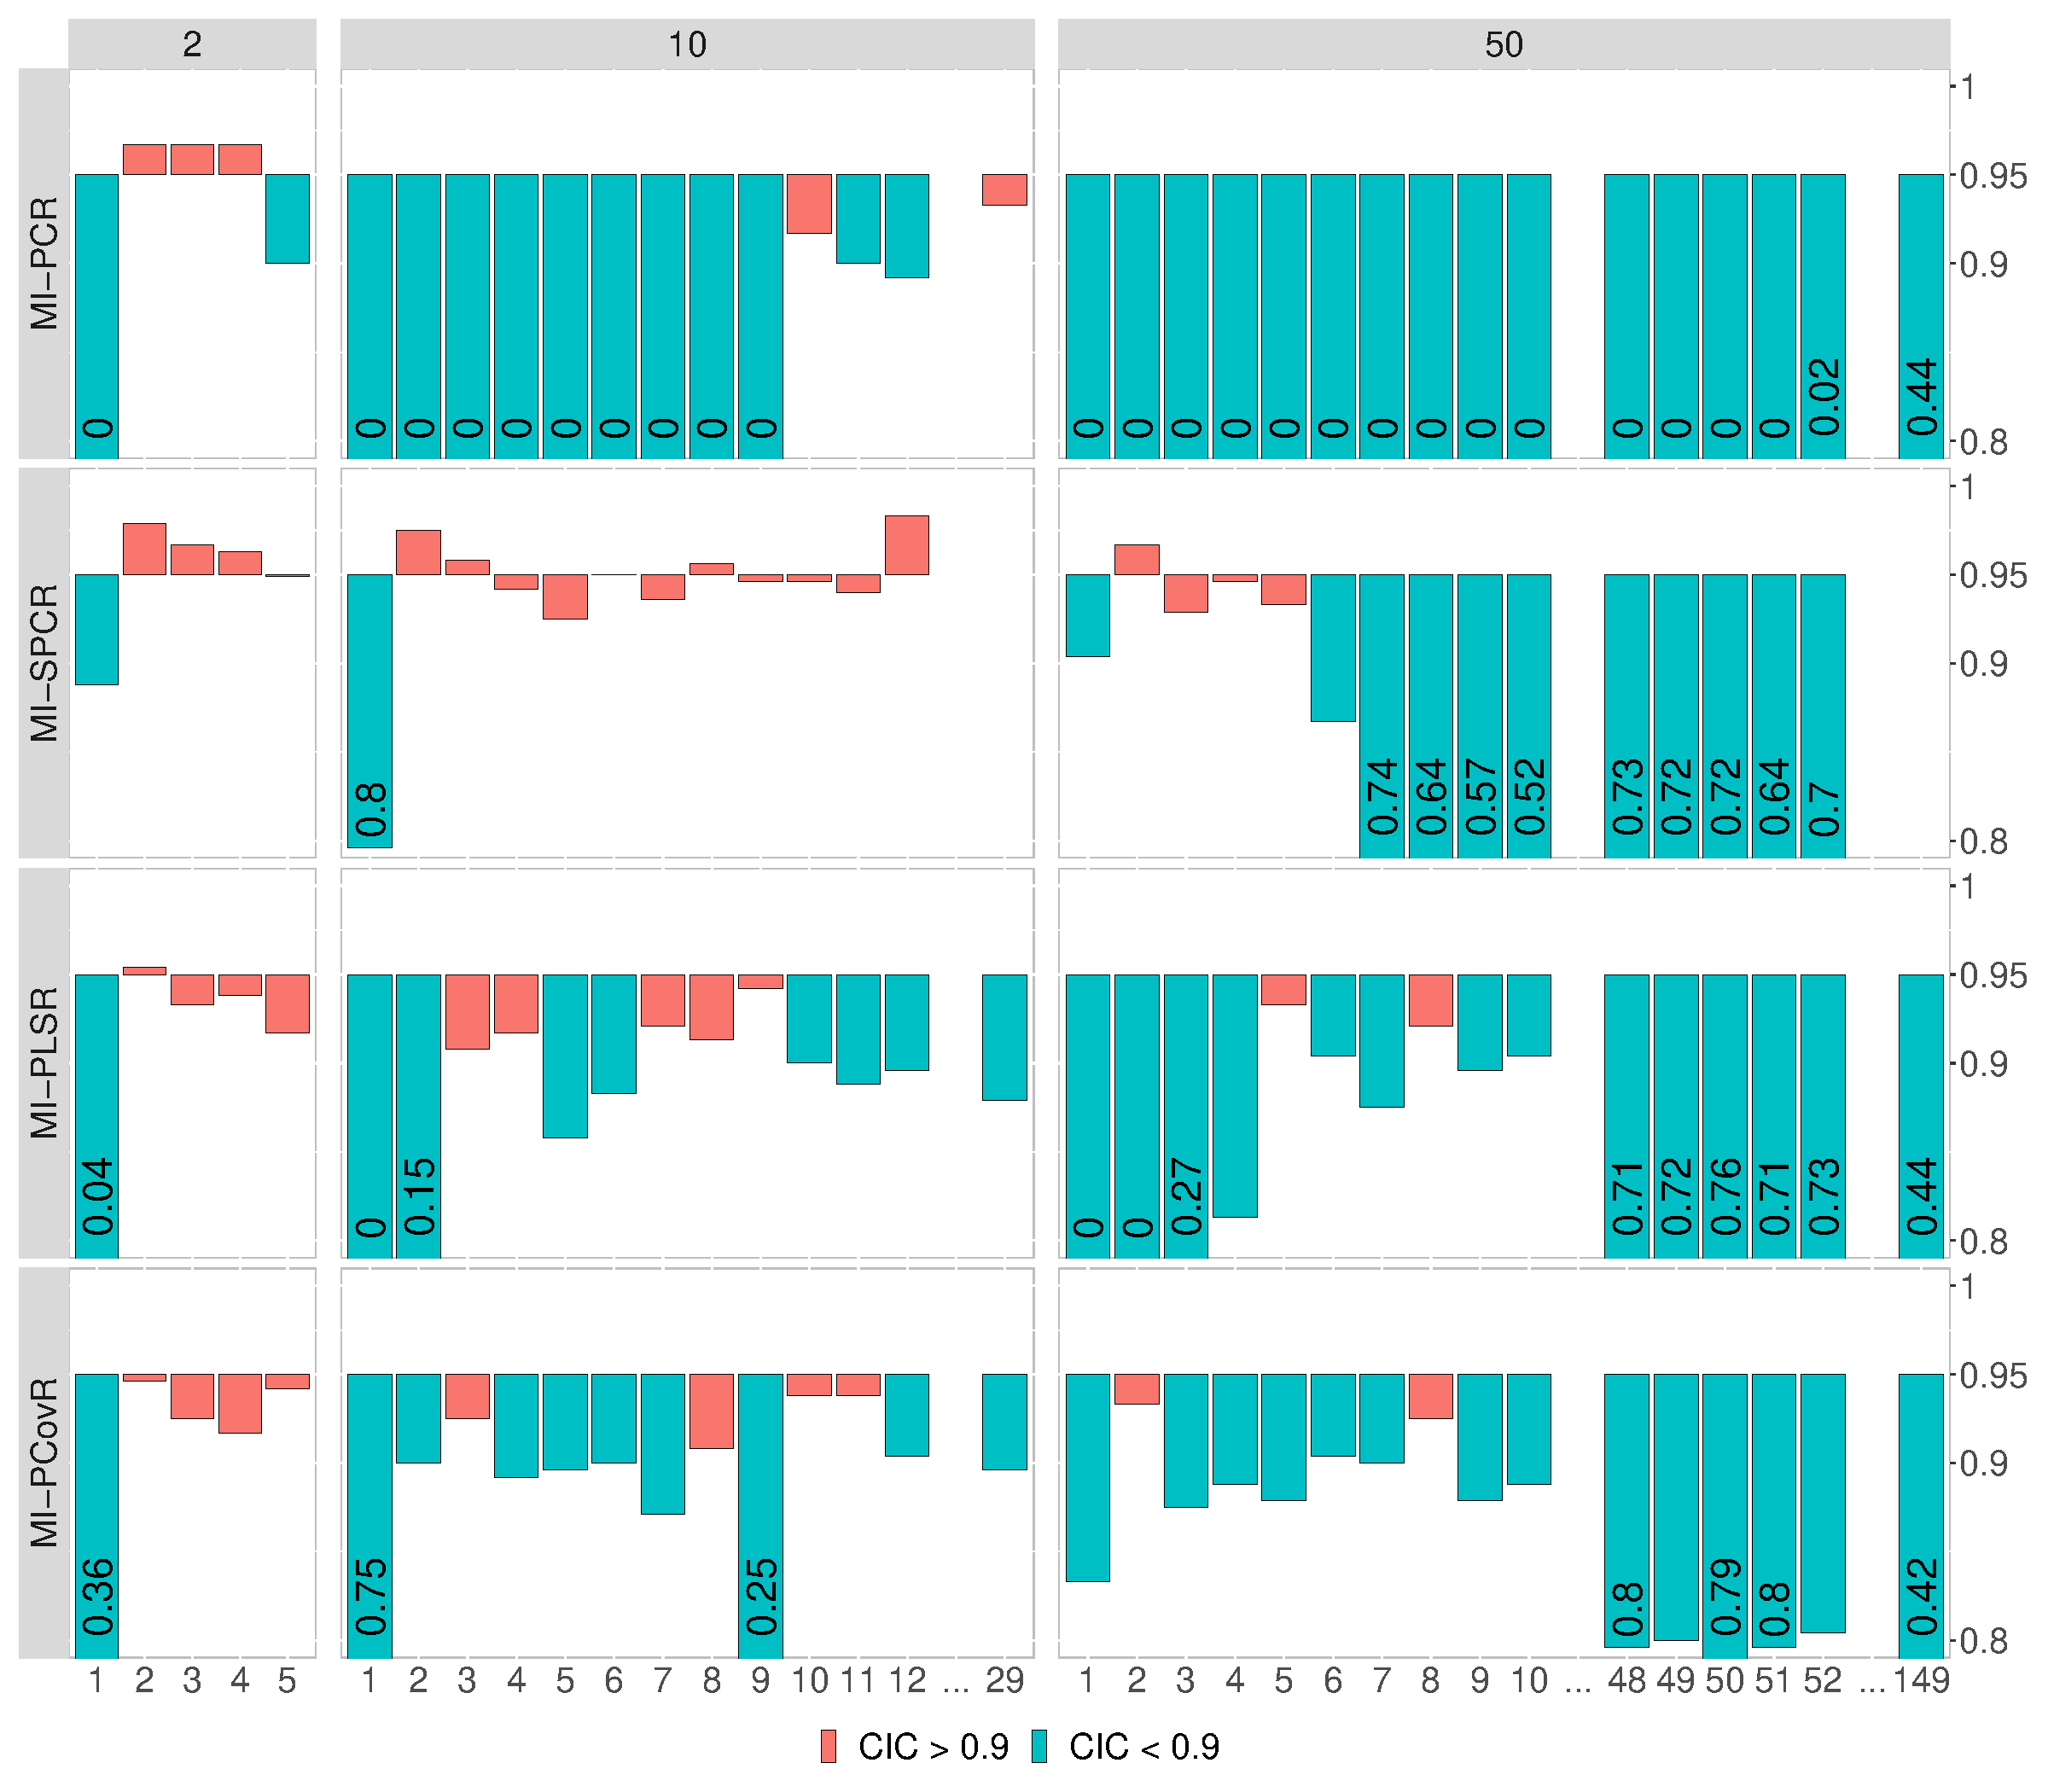
\includegraphics[width=\maxwidth]{figure/plot-cic-1} 

}


\end{knitrout}
          \caption{
            \label{fig:prb} 
            The confidence interval coverage for the correlation coefficient between $x_1$ and $x_2$, obtained after imputing the missing values with the four PCR-based imputation methods (grid rows), is reported as a function of the number of components used (X-axis).
            }
        \end{figure}
    
    \end{block}
    \end{column}

  \end{columns}

  \bigskip
  {\usebeamercolor[bg]{headline}\hrulefill}
  \bigskip

% Section 4 --------------------------------------------------------------------

\begin{columns}

  % First column
  \begin{column}{.28\textwidth}
    \begin{block}{Project summary and code}
      \begin{center}
        
\includegraphics[width = 15cm]{images/GitHub.png}
        \end{center}
    
      \end{block}
  \end{column}

  % Second column
  \begin{column}{.28\textwidth}
    \begin{block}{Play with the Shiny app}
      \begin{center}
        
\includegraphics[width = 15cm]{images/Shiny_app.png}
        \end{center}
  
    \end{block}
  \end{column}

  % Third column
  \begin{column}{.28\textwidth}
    \begin{block}{More research like this}
      \begin{center}
        
\includegraphics[width = 15cm]{images/Personal_website.png}
        \end{center}

    \end{block}
  \end{column}

  \end{columns}  

  \bigskip
  {\usebeamercolor[bg]{headline}\hrulefill}
  \bigskip


\end{frame}
\end{document}
